\problemname{Thousands Islands}

\begin{quote}
\textit{Note:} in this problem, you have to write your solution in C++.
\end{quote}

Thousands Islands is a group of beautiful islands located in the Java Sea. It consists of $N$ islands,
numbered from $0$ to $N-1$.

There are $M$ canoes, numbered from $0$ to $M-1$, that can be used to sail between islands. For each
$i$ such that $0 \leq i \leq M-1$, canoe $i$ can be docked either at island $U[i]$ or $V[i]$, and can
be used to sail between islands $U[i]$ and $V[i]$. Specifically, when the canoe is docked at island
$U[i]$, it can be used to sail from island $U[i]$ to island $V[i]$, after which the canoe becomes
docked at island $V[i]$. Similarly, when the canoe is docked at island $V[i]$, it can be used to sail
from island $V[i]$ to island $U[i]$, after which the canoe becomes docked at island $U[i]$. Initially,
the canoe is docked at island $U[i]$. It is possible that multiple canoes can be used to sail between
the same pair of islands. It is also possible that multiple canoes are docked at the same island.

For safety reasons, a canoe needs to be maintained after every time it is sailed, which forbids the
same canoe to be sailed two times in a row. That is, after using some canoe $i$, another canoe must be
used before canoe $i$ can be used again.

Bu Dengklek wants to plan a journey through some of the islands. Her journey is \emph{valid} if and
only if the following conditions are satisfied.
\begin{itemize}
  \item She starts and ends her journey at island $0$.
  \item She visits at least one island other than island $0$.
  \item After the journey ends, each canoe is docked at the same island as it was before the journey.
  I.e., canoe $i$, for each $i$ such that $0 \leq i \leq M-1$, must be docked at island $U[i]$.
\end{itemize}

Help Bu Dengklek find any valid journey involving sailing at most $2\,000\,000$ times, or determine
that no such valid journey exists. It can be proven that under the constraints specified in this task
(see the Constraints section), if a valid journey exists, there also exists a valid journey that does
not involve sailing more than $2\,000\,000$ times.

\section*{Implementation Details}
You should implement the following procedure:

\begin{verbatim}
std::variant<bool, std::vector<int>> find_journey(
        int N, int M, std::vector<int> U, std::vector<int> V)
\end{verbatim}

\begin{itemize}
  \item $N$: the number of islands.
  \item $M$: the number of canoes.
  \item $U$, $V$: arrays of length $M$ describing the canoes.
  \item This procedure should return either a boolean or an array of integers.
  \begin{itemize}
    \item If no valid journey exists, the procedure should return \texttt{false}.
    \item If a valid journey exists, you have two options:
    \begin{itemize}
      \item To be awarded the full score, the procedure should return an array of at most
      $2\,000\,000$ integers representing a valid journey. More precisely, the elements of this array
      should be the numbers of the canoes that are used in the journey (in the order they are used).
      \item To be awarded a partial score, the procedure should return \texttt{true}, an array of more
      than $2\,000\,000$ integers, or an array of integers not describing a valid journey. See the
      Scoring section for more details.
    \end{itemize}
  \end{itemize}
  \item This procedure is called exactly once.
\end{itemize}

Your submission must not contain a \texttt{main} function, and must not read from standard input or
write to standard output: a grader is compiled together with your submission and does that for you.
The declaration above lives in \texttt{islands.h}, which is available both to your submission and as
an attachment, so start your file with \texttt{\#include "islands.h"}.

\section*{Constraints}
\begin{itemize}
  \item $2 \leq N \leq 10^5$
  \item $1 \leq M \leq 2 \cdot 10^5$
  \item $0 \leq U[i] \leq N-1$ and $0 \leq V[i] \leq N-1$ (for each $i$ such that
  $0 \leq i \leq M-1$)
  \item $U[i] \neq V[i]$ (for each $i$ such that $0 \leq i \leq M-1$)
\end{itemize}

\section*{Scoring}
Your solution will be tested on a set of test groups.
For each test case in which a valid journey exists, your solution
\begin{itemize}
  \item gets full points if it returns a valid journey,
  \item gets $35\%$ of the points if it returns \texttt{true}, an array of more than $2\,000\,000$
  integers, or an array that does not describe a valid journey,
  \item gets $0$ points otherwise.
\end{itemize}
For each test case in which a valid journey does not exist, your solution
\begin{itemize}
  \item gets full points if it returns \texttt{false},
  \item gets $0$ points otherwise.
\end{itemize}
The score for a test group is the minimum of the points for the test cases in that group.

\noindent
\begin{tabular}{| l | l | p{12cm} |}
  \hline
  \textbf{Group} & \textbf{Points} & \textbf{Constraints} \\ \hline
  $1$ & $5$  & $N = 2$ \\ \hline
  $2$ & $5$  & $N \leq 400$. For each pair of distinct islands $x$ and $y$
               ($0 \leq x < y \leq N-1$), there are exactly two canoes that can be used to sail
               between them. One of them is docked at island $x$, and the other one is docked at
               island $y$. \\ \hline
  $3$ & $21$ & $N \leq 1000$, $M$ is even, and for each even $i$ such that $0 \leq i \leq M-1$,
               canoes $i$ and $i+1$ can both be used to sail between islands $U[i]$ and $V[i]$.
               Canoe $i$ is initially docked at island $U[i]$ and canoe $i+1$ is initially docked at
               island $V[i]$. Formally, $U[i] = V[i+1]$ and $V[i] = U[i+1]$. \\ \hline
  $4$ & $24$ & $N \leq 1000$, $M$ is even, and for each even $i$ such that $0 \leq i \leq M-1$,
               canoes $i$ and $i+1$ can both be used to sail between islands $U[i]$ and $V[i]$.
               Both canoes are initially docked at island $U[i]$. Formally, $U[i] = U[i+1]$ and
               $V[i] = V[i+1]$. \\ \hline
  $5$ & $45$ & No additional constraints. \\ \hline
\end{tabular}

\section*{Sample Grader}
A sample grader is available under ``attachments'' at the bottom of this page, together with
\texttt{islands.h} and the two sample inputs. Compile it with your solution and run it on an input
file to try your solution locally. It reads the input in the following format:
\begin{itemize}
  \item line $1$: $N$ $M$
  \item line $2 + i$ ($0 \leq i \leq M-1$): $U[i]$ $V[i]$
\end{itemize}
If \texttt{find\_journey} returns a \texttt{bool}, it prints
\begin{itemize}
  \item line $1$: $0$
  \item line $2$: $0$ if \texttt{find\_journey} returns \texttt{false}, or $1$ otherwise.
\end{itemize}
If \texttt{find\_journey} returns an array, denote its elements by
$c[0], c[1], \ldots, c[k-1]$. The sample grader prints
\begin{itemize}
  \item line $1$: $1$
  \item line $2$: $k$
  \item line $3$: $c[0]$ $c[1]$ $\ldots$ $c[k-1]$
\end{itemize}
That is the format of the sample data below. The sample grader does not check whether the journey is
valid; the judge does that.

\section*{Explanation of Sample 1}
In the first sample, $N = 4$ and $M = 5$. The islands and canoes are shown in the picture below.

\begin{center}
  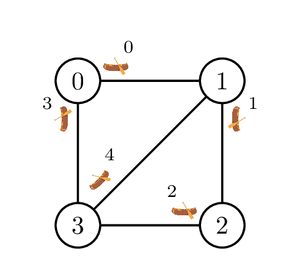
\includegraphics[width=0.33\textwidth]{islands-ex1.png}
\end{center}

One possible valid journey is as follows. Bu Dengklek first sails canoes $0$, $1$, $2$ and $4$ in that
order. As a result, she is at island $1$. After that, Bu Dengklek can sail canoe $0$ again as it is
currently docked at island $1$ and the last canoe she used is not canoe $0$. After sailing canoe $0$
again, Bu Dengklek is now at island $0$. However, canoes $1$, $2$ and $4$ are not docked at the same
islands as they were before the journey. Bu Dengklek then continues her journey by sailing canoes $3$,
$2$, $1$, $4$ and $3$ again. Bu Dengklek is back at island $0$ and all the canoes are docked at the
same islands as before the journey.

Therefore the sequence $0, 1, 2, 4, 0, 3, 2, 1, 4, 3$ represents a valid journey. Any other valid
journey is also accepted.

\section*{Explanation of Sample 2}
In the second sample, $N = 2$ and $M = 3$. The islands and canoes are shown in the picture below.

\begin{center}
  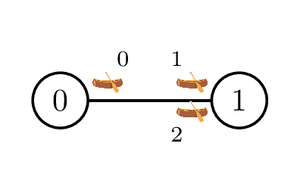
\includegraphics[width=0.33\textwidth]{islands-ex2.png}
\end{center}

Bu Dengklek can only start by sailing canoe $0$, after which she can sail either canoe $1$ or $2$.
Note that she cannot sail canoe $0$ twice in a row. In both cases, Bu Dengklek is back at island $0$.
However, the canoes are not docked at the same islands as they were before the journey, and Bu
Dengklek cannot sail any canoe afterwards, as the only canoe docked at island $0$ is the one she has
just used.

As there is no valid journey, the procedure should return \texttt{false}, which the sample grader
prints as $0$ followed by $0$.
